\documentclass[11pt,a4paper]{article}
\usepackage[margin=23mm]{geometry}
\usepackage[T1]{fontenc}
\usepackage{lmodern}
\usepackage{hyperref}
\usepackage{tikz}
\usetikzlibrary{positioning,arrows.meta}
\title{HyMeKo dependency refresh: approval boundary and sequence}
\date{Created-at: 2026-09-05 20:11 +02:00}
\begin{document}
\maketitle
\paragraph{Scope and acceptance.}
Continue the user's latest-provider, dependency-refresh and subsequent tagging
instructions in the existing checkouts. Core base: 7186b55. Core fetched at 20:10,
ahead 26 / behind 0; Parser fetched at 20:09. Proposed protected scope is only
Core Cargo.lock: parser e28a205147c48273980e63aa3338ca286974a6ed to
284c490d68232973a006bcba974279fed6f89ce8. The latter adds only Parser's own lock;
source and Cargo manifest are identical. Keep the existing master source identity.
\paragraph{Authorization.}
The original user task explicitly protects Core dependency changes and requires
an applicable literal token. Received in the user chat before implementation,
at this resumed task's 2026-09-05 20:45 +02:00 startup:
\texttt{APPROVED-CORE-EDIT: core-parser-latest-revision}.
The approving chat turn identifier is not exposed. The one-line patch was
prepared and checked before approval at 0c4e40a. Record this token in the scoped
dependency commit footer. The original distributed-admission token remains separate.
ETA: 5 minutes for the proposal; after approval 10--20 minutes for Core refresh
and clean Docker verification, based on the measured 82-second Core suite plus
image preparation. Broader consumer work gets measured per existing harness.
\paragraph{Discovery and affected files.}
Reuse Cargo's lock resolution, existing Dockerfile and tools/ci/core.sh. Core
Cargo.toml and hymeko\_core/Cargo.toml need no changes. The proposal adds this
quartet, reports/2026-09-05-dependency-refresh.md and
reports/dependency-refresh/core-parser.patch plus plan-build evidence.
Extend that same evidence directory with Cargo-update logs, source/bundle hashes,
image-build metadata and logs, final container/image inspect data, dependency
identity inventory, resource summary and a final execution artifact manifest.
Update docs/core-container.md's Parser pin documentation. Reuse the existing
Amaterasu clean/core checkout at 8a0c49d, updating it from a scoped Git bundle
only after clean status and base verification. The previous image remains intact;
the new commit gets its own image tag and a new empty target volume.
Use .gitattributes for exact evidence bytes if needed.
\paragraph{Provider to consumer continuation.}
After testing Core, record FINAL\_CORE. Align the exact same URL and Core rev in
Graph root Cargo.toml, Cargo.lock and benchmarks/Cargo.lock; Transformation root
Cargo.toml/lock; Hotaru root Cargo.toml/lock; Network root Cargo.toml/lock;
VSCode server/Cargo.toml/lock; Simulator root Cargo.toml/lock. Transformation
and Hotaru have their own final revisions for downstream consumers. Keep one
Parser source identity everywhere. Current Tensor is already fresh. Graph P34
feature integration is a separate pending scope choice; do not discard the two
platform correctness patches or merge feature code under a dependency-only scope.
\paragraph{Tests, invariants and rollback.}
Use cargo update with the exact Parser commit and inspect the one-line lock delta.
Verify one Core and Parser identity with cargo tree --locked -d. Build the existing
clean-source Core SDK on Amaterasu and run its all entry point under 16 GiB,
no additional swap, six CPUs. Require full Core tests, nine admission regressions,
CBOR corpus, formatting, Clippy and smoke checks; keep fixture/hash expectations.
The Lean source is unchanged, so reuse its valid proof artifact. Check affected
consumer tests, Graph's separate benchmark workspace, Simulator ingress and WASM
before claiming integration. No API, IR, wire, grammar or numerical change.
Rollback only the scoped dependency commit, retaining its previous lock revision.
\paragraph{Consumer execution boundary, 2026-09-05 21:14 +02:00.}
FINAL\_CORE is ac1131b5490734b855021f6076753417e1337cd6, published on the
existing audit feature branch. Its runtime sources and lock are identical to the
clean-image verified implementation 1886f17. Reuse that SDK image for consumer
checks. Amaterasu cannot mount the Windows worktrees, and discovery found no
task-owned Graph or Transformation checkout there. Therefore create clean,
task-owned checkouts under the existing distributed-admission task directory's
dependency-refresh/consumers area from scoped Git bundles. This physical host
boundary is the reason for the extra checkouts; they are disposable verification
copies, not new implementation worktrees. Retain them with the evidence until the
task is accepted. Reuse the SDK's Cargo registry in one task-owned Cargo volume;
fetch private Git dependencies with an ephemeral forwarded SSH socket and strict
known-host checking. Fetch containers and offline test containers each have a
16 GiB memory cap, zero swap and six CPUs. Each consumer starts with an empty
target volume. No permanent alternate runner or Dockerfile is introduced.
Run existing workspace tests with --release --locked, Graph's existing governance
gate against its committed revision, and cargo bench --no-run in Graph's separate
benchmark workspace. Inspect locked metadata for one canonical Core and Parser
identity. Record raw logs, timings, cgroup memory peak and container exit status
in each consumer's reports/dependency-refresh directory. ETA: 10--15 minutes for
the two consumers, dominated by fresh compilation. Formatting and Clippy are
diagnostic for this dependency-only change; do not rewrite unrelated source to
absorb pre-existing lint failures.
Apply the same physical-boundary checkout exception and bounded SDK containers
to Hotaru, Network and VSCode/LSP under that consumers area, each from its own
scoped dependency commit. Reuse the shared Cargo download volume; use an empty
target volume per repository. Hotaru must pass both its default tests and its
hymeko-ir feature tests; Network runs its full tests and LSP its server tests.
The tested Transformation and Hotaru commits must be published on authorized
feature branches before downstream lock resolution, without local path overrides.
Record these smaller consumer results in the existing central evidence package.
\paragraph{Required consumer API adaptation, 21:27 +02:00.}
The first Hotaru feature-enabled build reproduced three removed/private Core
field accesses in src/hypergraph/ir.rs. Extend only the existing adapter to use
Ir::arc, Ir::as\_node and Id::raw. Existing tests/ir\_hypergraph.rs already checks
compiled signs, qualified names, incidence and containment. Preserve the
dependency-free default and require both existing feature configurations.
Network has the analogous obsolete declaration maps only in its existing
src/model.rs test builder; when that dependency stage is reached, replace those
manual mappings with push\_decl and bind\_node\_decl/bind\_edge\_decl, preserving
the intentional malformed fixtures and explicit decl\_hash entries. Core owns
these public APIs and needs no change. No new tests or compatibility layer are
needed for this mechanical adaptation. Rollback each consumer's separate
adapter commit together with its dependency commit, leaving other owners intact.
\paragraph{Discovered modal verification defect, 21:29 +02:00.}
The fixture-enabled Transformation suite fails the existing six-body closed-form
spectrum test: a numerical residue at an exact zero root is reported as a
seventh positive-frequency mode. This blocks the consumer verification gate.
Keep its correction in a separate Transformation commit, outside Core. Discovery
found the sole eigenvalue owner in hymeko\_dynamics/src/analysis.rs and the existing
many\_body integration test file. Confirm the chain's computed constant
coefficient is exactly zero before applying the correction. For the already
computed polynomial, factor only exactly zero trailing coefficients:
$p(\lambda)=\lambda^z q(\lambda)$. Run the existing solver on $q$, append $z$
exact complex zeros, and retain the full trace/determinant checks. Handle the
degree-zero case without calling the iterative solver. Preserve every nonzero
coefficient and the existing modal tolerance; introduce no new public API.
Extend that existing test file with closed-form null matrices and oscillator
blocks, tiny nonzero frequencies, power-of-two scaling and coordinate
permutations. Require the original chain spectrum tolerance unchanged, then
the full fixture-enabled workspace suite. Retain pre-fix failures and the
fixture-free early-return diagnostic explicitly as invalid validation evidence.
This is a bounded zero-root correction, not a certificate for arbitrary dense
eigenproblems; conditioning and coefficient underflow remain existing limits.
ETA: 10 minutes. Rollback the standalone modal commit; keep dependency and
verification evidence distinct. Reuse the existing target/cache and bounded
Amaterasu SDK containers for the affected checks.
\paragraph{Final local consumer snapshot boundary.}
The existing Simulator integration snapshot is local-only, with no remote. Its
Chordex and XR path dependencies are likewise local snapshots. Reuse those exact
owners and revisions; do not publish invented upstreams. For Amaterasu verification
only, transfer their committed Git snapshots into the same task-owned consumers
area as hymeko\_simulator, soma\_chordex and xr so the existing relative paths
resolve. Replace only Core/WebXR task-local paths and Core patch override with
the tested published Core and Transformation Git revisions. Keep the existing
Chordex/XR paths explicitly local-only. Reuse the SDK with a task-owned rustup
volume seeded from the image; install wasm32-unknown-unknown in a bounded fetch
container. Require the existing Simulator model\_ingress suite with
--no-default-features --features zenoh-ingress, and cargo check --lib --target
wasm32-unknown-unknown --no-default-features, both --locked --offline. These gates
verify the updated dependency closure; real browser transport remains the separate
consumer experiment. Record source revisions, locked identities and resource
evidence centrally. ETA: 5--10 minutes including fresh dependency compilation.
\paragraph{Publication and tags.}
Local revision closure does not establish remote availability. Consumers cannot be
reported portable until every referenced revision is reachable at its configured
source and verification succeeds without task-local overrides. Tag only the tested
revision set after the user's requested order; do not invent a release version,
publish tags, merge main or push unpublished revisions without the needed scope.
\paragraph{Remaining branches audit, 2026-09-06 00:22 +02:00.}
The user now requests inspection of the excluded branches. Reuse this plan and
the central dependency report. Fresh refs: Core audit 89d221f versus semantic
digest 112a254 (16/5 commits); Graph audit 4a59c23 versus P34 83774b8 (4/49).
Git merge-tree may write unreachable objects but must not change a working tree,
index or branch. Core's conflict-free result includes portable ID serialization
and three robotics commits; inspect these separately from the seven-file digest
commit. Graph has four textual conflicts and needs semantic reconciliation.
No protected implementation edit, dependency update, integration commit or tag
is authorized by this diagnostic step. The earlier slug-specific approvals do
not cover a new digest implementation or wire change.

Use existing incoming tests before extending the test-only diagnostic surface.
Discriminate deep-value truncation and declaration/arc renumbering with minimal
counterexamples; retain expected failures. A further coverage control changes
an edge-owned ArcRec target without a separate HyperArc declaration; require
both CBOR encode/decode acceptance and a changed V1 structure hash before
asserting that V2 must differ. Check the corpus-golden attribution
by running the same test binary with incoming and audit data trees: changing
fixtures must not be misreported as a hash-algorithm change. No frozen hash is
updated. Incoming branch tests are diagnostic evidence, not merged-suite results.

Reuse Amaterasu's existing clean/core object store and Core SDK image 1886f17.
Transfer a scoped Git bundle into the existing dependency-refresh directory,
fetch its objects without checkout, and extract the incoming committed source
only inside a disposable bounded container. This is a physical-host verification
copy, not a new implementation worktree. Preserve all existing checkouts, images
and tags. Mount the shared Cargo cache and reuse an appropriate Core target
cache; 16 GiB memory, no extra swap, six CPUs, offline test execution. Add no
dependencies. Archive the exact test-only patch, source refs, raw output,
container exit and memory peak under reports/dependency-refresh; retire the
temporary source with the stopped diagnostic container after task acceptance.

ETA: 10--15 minutes, based on the previous 84-second cold Core gate plus focused
rebuild and report preparation. No performance claim or full benchmark rerun.
Acceptance is an evidence-backed integration order, exact conflicting files,
protected scope, invariants, focused and full future gates, and rollback.
Rollback of this audit is limited to its documentation/evidence additions;
actual integration, if later approved, uses separate thematic commits and keeps
the current tested consumer revision set available unchanged.
\begin{center}
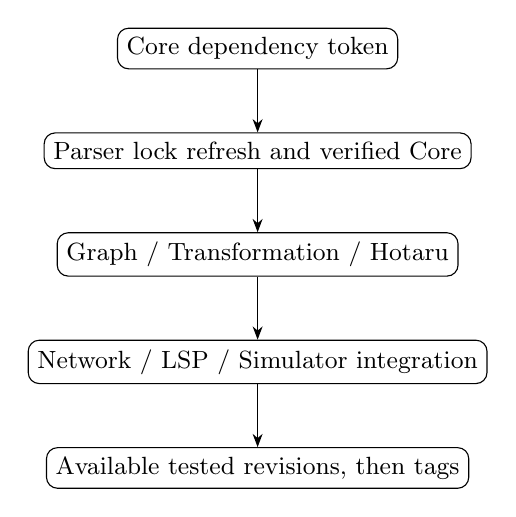
\begin{tikzpicture}[node distance=8mm, every node/.style={draw,rounded corners,align=center,font=\small}, >={Stealth}]
\node (a) {Core dependency token};
\node (c) [below=of a] {Parser lock refresh and verified Core};
\node (o) [below=of c] {Graph / Transformation / Hotaru};
\node (u) [below=of o] {Network / LSP / Simulator integration};
\node (t) [below=of u] {Available tested revisions, then tags};
\draw[->] (a)--(c); \draw[->] (c)--(o); \draw[->] (o)--(u); \draw[->] (u)--(t);
\end{tikzpicture}
\end{center}
\begin{center}
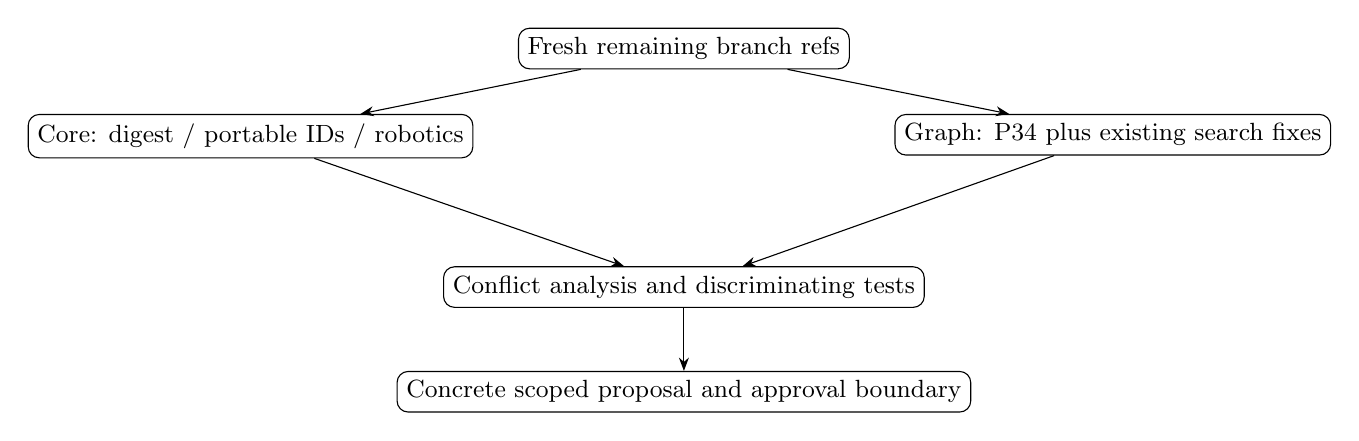
\begin{tikzpicture}[node distance=8mm, every node/.style={draw,rounded corners,align=center,font=\small}, >={Stealth}]
\node (r) {Fresh remaining branch refs};
\node (s) [below left=of r] {Core: digest / portable IDs / robotics};
\node (g) [below right=of r] {Graph: P34 plus existing search fixes};
\node (v) [below=25mm of r] {Conflict analysis and discriminating tests};
\node (a) [below=of v] {Concrete scoped proposal and approval boundary};
\draw[->] (r)--(s); \draw[->] (r)--(g); \draw[->] (s)--(v); \draw[->] (g)--(v); \draw[->] (v)--(a);
\end{tikzpicture}
\end{center}

\end{document}
